\chapter{Systembeskrivelse}\label{ch:Systembeskrivelse}
Systemet BargainBarter er en Webapplikation, der hostes på \url{http://10.29.0.30/BargainBarter} på IHA's netværk. Denne hjemmeside tilbyder brugere at oprette en brugerprofil, hvorefter de for mulighed for at benytte kernen af hjemmesidens funktionaliteter.
En af kernefunktionaliteterne er at kunne oprette en bytteannonce, med det formål at kunne bytte denne med en andens brugers bytteannonce. Annoncen er simpel i den forstand at den består af et billede, en titel, en beskrivelse og en kategori. Når denne annonce er oprettet bliver det muligt for andre brugere af hjemmesiden at se den i det samlede overblik over annoncer på forsiden og klikke ind på den for nærmere detaljer. Herfra har en bruger adgang til informationer om sted/adresse på den tilhørende bruger på bytteannoncen, afstand til den tilhørende bruger, offentlige kommentarer på annoncen, den tilhørende brugers byttehistorik og vurderinger fra andre brugere på baggrund af tidligere byttehandler.
Brugeren har tilgang til et fælles chatrum, hvor man evt. kan skrive om tid og sted for byttehandlen. \\

\noindent En rigt billede, der illustrer systemets primære funktionalitet kan ses på figur \ref{fig:rigbillede} hvor et simpel byttescenarie gennemføres.

\begin{figure}[H]
	\centering
	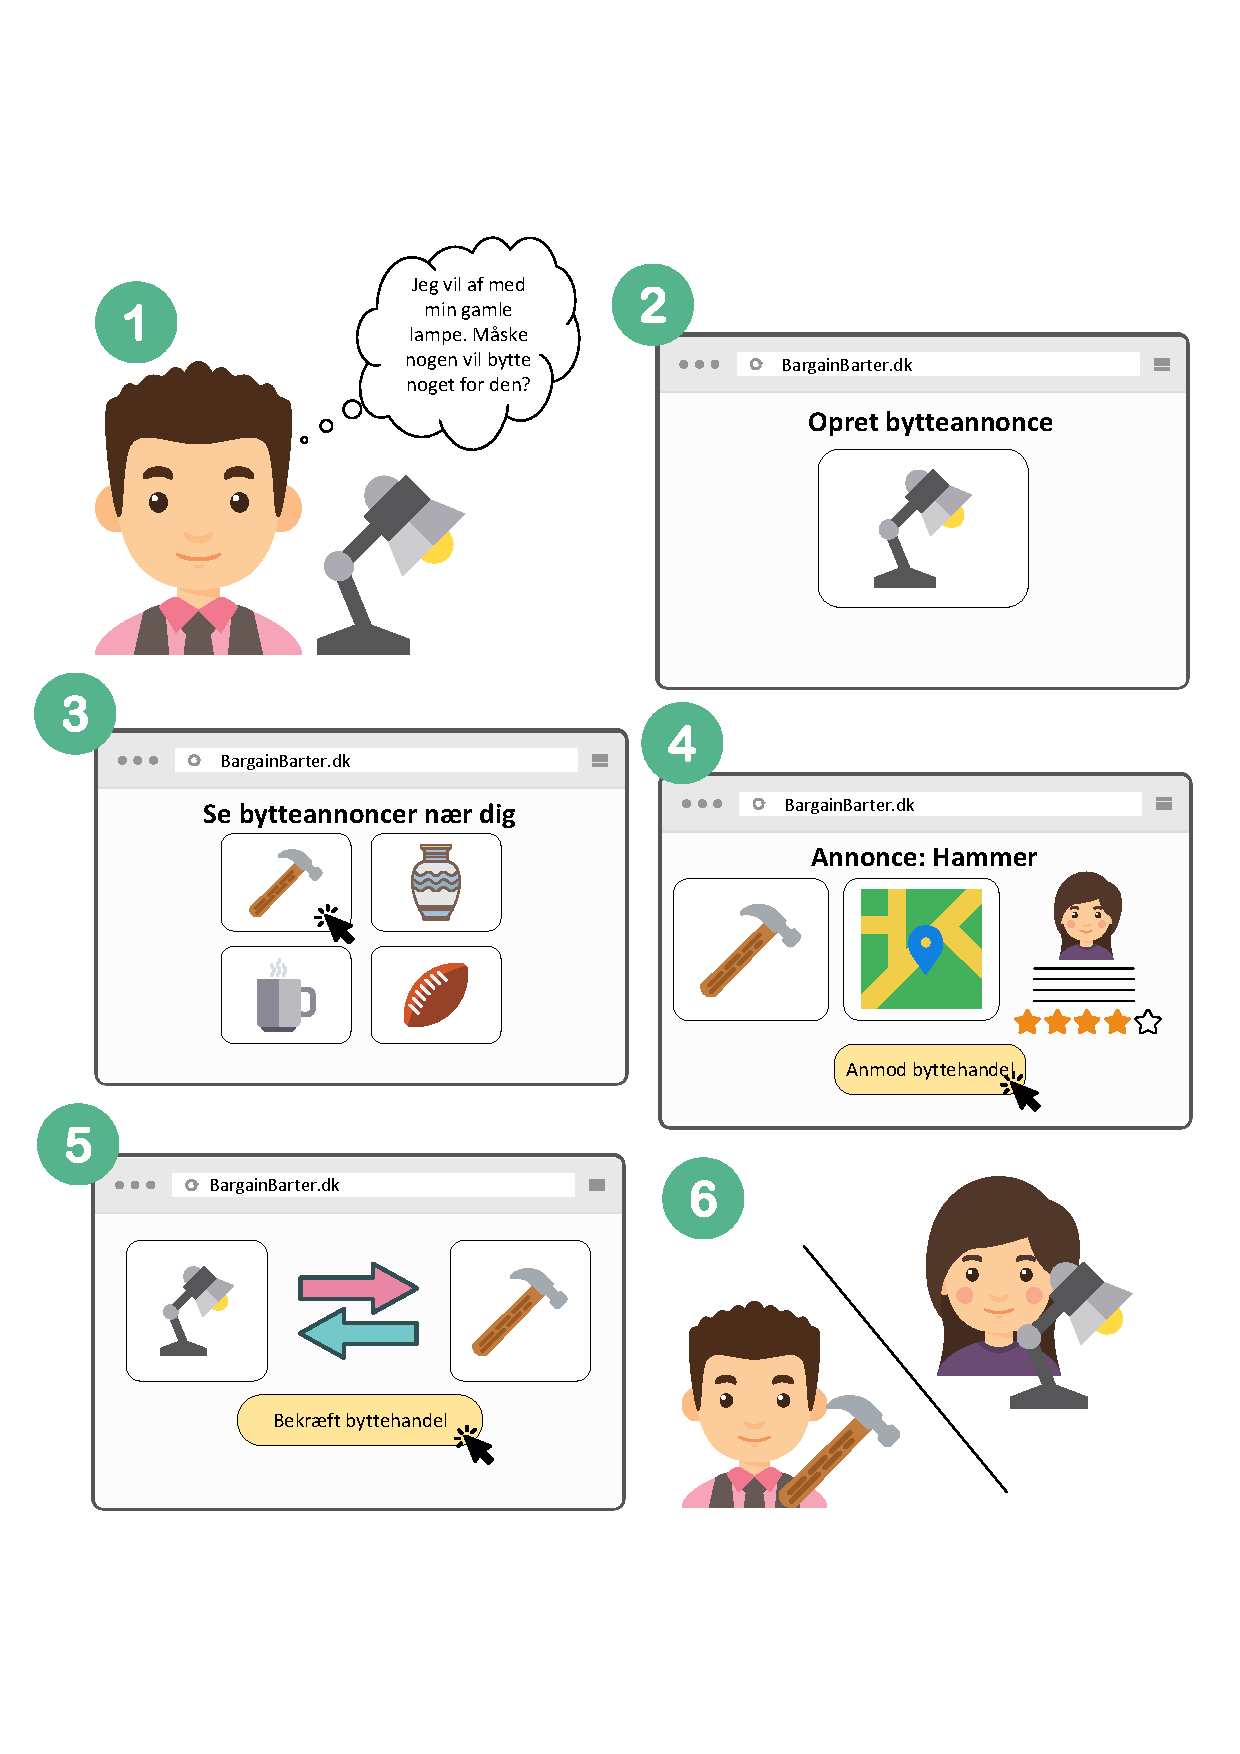
\includegraphics
	[width=140mm]{figures/rigtbillede_version1.pdf}
	\caption{Rigt billede}
	\label{fig:rigbillede}
\end{figure} 

På figuren ses det, at byttehandlerne  bekræftes eller afvises  direkte i systemet. Derfor skal du, for at få værdi af systemet, som bruger gennemføre byttehandlen i virkeligheden efter bekræftelsen og derefter bekræfte at byttehandlen har fundet sted. 